\documentclass[12pt,a4paper]{article}
\usepackage[margin=2.5cm]{geometry}
\usepackage{amsmath,amssymb,amsthm}
\usepackage{graphicx}
\usepackage{booktabs}
\usepackage{xcolor}
\usepackage[colorlinks=true,linkcolor=blue!60!black,citecolor=blue!60!black,urlcolor=blue!60!black]{hyperref}
\usepackage[numbers]{natbib}
\usepackage{caption}
\captionsetup{font=small,labelfont=bf}
\emergencystretch=2.5em

\newtheorem{proposition}{Proposition}
\newcommand{\etav}{\eta_v}
\newcommand{\etar}{\eta_r}
\newcommand{\etag}{\eta_g}
\newtheorem{definition}{Definition}
\newtheorem{remark}{Remark}

\title{Maneuvering Formations in Directional Fields:\\
Path-Integrated Exposure and Delayed Threats\\
in Nonholonomic Adversarial Games}
\author{Research Layer of the \emph{Iron Bottom Sound} project\thanks{All
experiments are reproducible from repository scripts against a frozen
deterministic rules engine (commit \texttt{fc77a65}).  The WWII surface-combat
wargame serves only as an external case study; this paper's
claims are about the general model class.}}

\date{September 11, 2026}

\begin{document}
\maketitle

\begin{abstract}
We study adversarial trajectory optimization between two moving
\emph{formations} that interact through a directional field under
nonholonomic motion constraints.  The decision variable is not a position but
a trajectory, and the objective is the path-integrated net exposure built
from a calibrated anisotropic interaction kernel; we characterize the
resulting closed-loop dynamic game and test its mechanisms numerically.
Three results are proved and measured.  First, the path-integrated objective
is load-bearing: snapshot and peak positional surrogates reorder committed
plans and can reverse a whole-trajectory ranking in a constructed example.
Second, a symmetric closed-loop degeneracy: under explicit player-exchange
symmetry the game value collapses exactly to the instantaneous payoff, while
capability monotonicity holds for nested maximum-speed sets.  Third, formation
representation matters as a robustness layer: the numerical naval
instantiation uses a leader--follower line-ahead formation in which trailing
vessels follow the leader's track at fixed arc-length offsets, and the
comparative statics tested here are unchanged when the rigid baseline is
substituted.  We also report a matched-horizon replanning experiment that
fixes the evaluation horizon and varies only the replanning cadence: the
earlier, horizon-confounded indication that longer commitment favors the
range-advantaged side does \emph{not} survive the correction, so we remove
commitment as a claim and report the corrected experiment as a negative
result with its control diagnostic.  Delayed threats act through
response-space contraction, with coverage and local intensity interacting
rather than either acting alone.  Finally, a matched external test in an
auditable rules engine shows that transfer of the reduced model's point
values is partial, which locates the boundary of the reduced model and makes
the engine an external case study rather than a validation claim.
\end{abstract}

\section{Introduction}\label{sec:intro}

How should an adversarial formation maneuver when the interaction strength
is directional, the motion is nonholonomic, and some controls have delayed
effects?  The classical naval answer --- cross the enemy's line to concentrate
broadside fire while presenting only bow or stern arcs --- is a doctrine about
\emph{positions}.  This paper argues that positions are the wrong primitive.
What matters is the \emph{cumulative interaction along trajectories}: the
path-integrated net exposure an opponent suffers versus the exposure one must
sustain in return.  From this vantage, crossing the T is merely one geometric
state that may or may not raise the integral --- never an objective in itself.

We develop this view on a complete, auditable wargame engine (deterministic conditional on sealed orders and random seed)
(\emph{Iron Bottom Sound}, IBS): a hexagonal WWII surface-combat simulation
whose adjudication is a pure function of state, sealed orders, and seed, with
every die roll audited against its rule reference.  The engine provides the
calibration target for our interaction field and the case-study environment for
our policies; the mathematical claims are about the model class, not the
wargame.  The resulting pipeline is:
\begin{enumerate}
\item calibrate a smooth anisotropic interaction kernel against the engine's
exact adjudication (retained fidelity $\rho=0.991$);
\item embed the kernel in a committed-maneuver dynamic game over
path-integrated exposure;
\item characterize the structural properties (the degeneracy boundary and
speed-capability monotonicity) and test a commitment-type comparative static
that the fixed-horizon correction subsequently removes;
\item translate model policies back into legal engine orders and validate
against doctrine baselines with paired seeds.
\end{enumerate}
Each step is gated by pre-specified acceptance criteria and every number in
this paper traces to a script in the repository.

\subsection{Contributions}
\begin{enumerate}
\item \textbf{A path-integrated anisotropic formation-game formulation}
for moving formations (\eqref{eq:formation}--\eqref{eq:ffield}): we show that
snapshot positional quality can reorder committed plans and can reverse a
whole-trajectory ranking, so the integral --- not the best position --- is the
object of optimisation.  The interaction kernel is calibrated against an
auditable rules engine ($\rho=0.991$, nMAE $5.7\%$), and an isotropic
ablation shows that removing directionality reduces held-out rank correlation
from $0.991$ to $0.952$.
\item \textbf{Structural closed-loop results under explicit symmetry
assumptions}: a symmetric closed-loop degeneracy with a complete proof
(skew-symmetric successor matrices collapse the value onto the instantaneous
payoff; the collapse is an interaction-symmetry phenomenon, untouched by
kinematic asymmetry), and maximum-speed capability monotonicity by nesting.
\item \textbf{A delayed spatiotemporal threat formulation} in which
response-space contraction depends jointly on threat coverage and local
intensity, with the near-optimal response set as the mediating object.
\end{enumerate}

\noindent The leader--follower formation used for the numerical
instantiation is a fidelity layer rather than an algorithmic contribution,
and the rules-engine study is an external case study, not a validation claim.
We additionally report, as a negative result, that a commitment--range
comparative static which appears in a horizon-confounded open-loop
experiment does not survive a matched-horizon replanning experiment
(Section~\ref{sec:commitment}).

\section{Related Work}\label{sec:related}

\subsection{Dynamic and differential games}
Zero-sum differential games originate with Isaacs' method of characteristics
\cite{isaacs1965}; the theory of feedback (closed-loop) versus open-loop
information structures and their associated Nash values is developed in
\cite{basar1999}.  Classical pursuit--evasion and combat models optimize
terminal capture, separation, or energy-style objectives; Lanchester-type
attrition and its optimal-control treatment \cite{taylor1974} and
PDE combat models \cite{protopopescu1989} aggregate force levels rather
than adjudicate anisotropic single-weapon interactions.  Our point of
departure is the objective: a \emph{path-integrated anisotropic
interaction} --- the cumulative net exposure along whole trajectories ---
for which instantaneous geometry is only an ingredient, not the prize.

\subsection{Reachability and viability}
Reachable-set and viability-kernel methods characterise states a system
can maintain under constraints \cite{aubin1991}, with Hamilton--Jacobi
reachability providing adversarial variants for continuous dynamic games
\cite{mitchell2005}.  In that literature the target set is given ex
ante.  Here the ``favorable region'' is itself defined by the directional
interaction value ($L\ge\alpha$), and reachability questions are coupled
to a path-integrated payoff: we ask not only whether a state is reachable
or invariant, but what sustaining it is worth along the trajectory.

\subsection{Commitment and information structure}
The strategic value of binding oneself --- committing to a plan the
opponent can observe --- is classical \cite{schelling1960}; in dynamic
games it separates open-loop from feedback equilibria \cite{basar1999},
and receding-horizon control makes the replanning cadence a design
variable \cite{mayne2000}.  Algorithmically, our open-loop solver is a
double-oracle scheme in the spirit of \cite{mcmahan2003}.  What this paper
adds to that literature is the treatment of \emph{formation-level}
trajectories in an adversary's directional field with a path-integrated
payoff, together with an explicit negative finding about a commitment-type
comparative static: an effect that appears when plan length and evaluation
horizon vary together does not survive once the horizon is held fixed
(Section~\ref{sec:commitment}).

\subsection{Leader--follower formation control}
Path-following formation control and vehicular platooning study exactly the
rule used here as the naval instantiation: a designated leader generates a
track and followers regulate along-path offsets and adopt the local tangent
\cite{skjetne2005, dunbar2006}.  That literature asks how to track a given
path with bounded spacing error; we use the same representation but ask a
game-theoretic question --- which path to choose when an adversary's
directional field and delayed weapons make the payoff path-integrated.  The
distinction matters for interpretation: fixed-offset and path-following
representations are \emph{different formation models}, not two
discretisations of one model, which is why the robustness section reports
both rather than assuming equivalence.

\subsection{Interdiction and spatiotemporal hazards}
Time-dependent shortest paths \cite{orda1990} and network interdiction
\cite{israeli2002} study adversaries who add costs to arcs or destroy
links.  Robust path planning around dynamic obstacles treats hazards as
spatial fields to avoid.  The delayed threat studied here differs
mechanically: a launched weapon is a \emph{stateful spacetime field} that
does not merely add path cost but reshapes the opponent's set of
near-optimal future responses --- a response-set contraction measured
against the near-optimal landscape, not against feasibility.

\section{General Formation Game}\label{sec:model}

\noindent\textbf{A player controls a formation, not a vessel.}  Throughout,
each player $i\in\{B,R\}$ commands a moving \emph{formation}: a designated
leader state together with a formation map that places the remaining
vessels.  Write $\mathcal H_i(t)$ for the leader history (position, heading,
speed and the path traversed so far) and let vessel $k$ of formation $i$
occupy
\begin{equation}
X_{ik}(t) \;=\; \mathcal G_{ik}\bigl(\mathcal H_i(t)\bigr),
\label{eq:formation}
\end{equation}
for a formation map $\mathcal G_{ik}$.  The leader obeys nonholonomic
kinematics, $\dot x_i=v_i\cos\psi_i$, $\dot y_i=v_i\sin\psi_i$,
$\dot\psi_i=\omega_i$, with $v\le\bar v_i$ and
$|\omega_i|\le\bar\omega$ (a minimum turn radius
$R_{\min}(v)=v/\bar\omega$ couples speed and turning).  Lateral
displacement therefore requires first rotating the velocity vector --- the
defining nonholonomic cost.

Equation~\eqref{eq:formation} deliberately leaves the formation map free.
Two instantiations are used in this paper:
\begin{equation}
\underbrace{\mathcal G^{\mathrm{R}}_{ik}
      = c_i + R(\psi_i)\,p_{ik}}_{\text{rigid baseline (fixed offsets)}},
\qquad
\underbrace{\mathcal G^{\mathrm{LF}}_{ik}
      = \gamma_i\bigl(s_i - \ell_k\bigr)}_{\text{leader--follower (path following)}},
\label{eq:two-maps}
\end{equation}
where $\gamma_i$ is the leader's arc-length parameterised track, $s_i$ the
leader's arc length and $\ell_k$ the vessels' arc-length offsets.  The rigid
map is analytically transparent and is treated as a baseline; the
path-following map is the main numerical instantiation
(Section~\ref{sec:naval}), because a line-ahead column of real ships follows
the leader's track through a turn instead of rotating as one body.  The
structural results below are stated for the general map: they require only
the stated symmetry assumptions on the induced game, not a particular
$\mathcal G$.  No experiment in this paper supports a claim about isolated
single vessels.

\noindent\textbf{Anisotropic formation field.}  Each vessel projects an
interaction kernel that depends on range, relative bearing, the two vessels'
headings, and capability state; because vessels of the same formation may
carry different headings under $\mathcal G^{\mathrm{LF}}$, the kernel is
indexed by the shooter's own heading $\psi_{ik}$.  The formation field
aggregates over its vessels,
\begin{equation}
F_i(x,t) \;=\; \sum_{k\in i} K_{ik}(x,t),
\label{eq:ffield}
\end{equation}
and formation-vs-formation interaction sums over vessel pairs.  In the
naval instantiation $K$ is the calibrated kernel of
Section~\ref{sec:kernel} and each formation is a line-ahead column.

\begin{proposition}[Formation aggregation]\label{prop:agg}
For rigid formations, formation-to-formation exposure is exactly additive
over vessel pairs:
\[
E_{i\to j}\;=\;\int_0^T F_i\bigl(x_j(t),t\bigr)\,dt
\;=\;\sum_{k\in i}\sum_{m\in j}\;
\int_0^T K\bigl(x_{jm}(t);\,x_{ik}(t),t\bigr)\,dt .
\]
\end{proposition}
\begin{proof}
By \eqref{eq:ffield} the formation field is a sum of per-vessel kernels,
and the integral is linear.  Hence the exposure of vessel $m$ of
formation $j$ equals the sum, over the vessels $k$ of formation $i$, of
the pairwise terms; summing over $m\in j$ gives the stated identity.
\end{proof}

\noindent This elementary identity pins down what ``formation payoff''
means operationally: the double sum over vessel pairs that all solvers in
this paper evaluate.

\noindent\textbf{Path-integrated objective.}  Against trajectory $x_j(t)$,
the cumulative exposure is $E_{B\to j}=\int_0^T F_B(x_j(t),t)\,dt$, and the
net path value is
\begin{equation}
J_{\text{gun}} \;=\; E_{B\to R} \;-\; \lambda\, E_{R\to B},
\qquad \lambda = 1.
\label{eq:J}
\end{equation}
The object of optimisation is not a position but a trajectory: the integral
is the primitive.  Discretely, $J=\sum_t \Delta t\,[P_{B\to R}(t)-\lambda
P_{R\to B}(t)]$ with formation-aggregate $P$ from \eqref{eq:ffield}.

\noindent\textbf{Delayed threat state.}  Torpedoes are not damage terms but a
delayed stateful field: the state extends to $z_t=(s_t,q_t)$, where $q_t$
records every launched weapon's position, heading, speed, remaining range,
and threat probability.  The spatiotemporal hazard $H(x,t;q_t)$ is generated
by past launches and constrains future responses (Section~\ref{sec:threat}).

\noindent\textbf{Information and commitment.}  In the closed loop both sides
re-optimize every step against current state.  In the committed (open loop)
game both sides seal formation heading plans of horizon $H$ before execution
--- mirroring the engine's sealed-order discipline.


\begin{figure}[!htb]
\centering
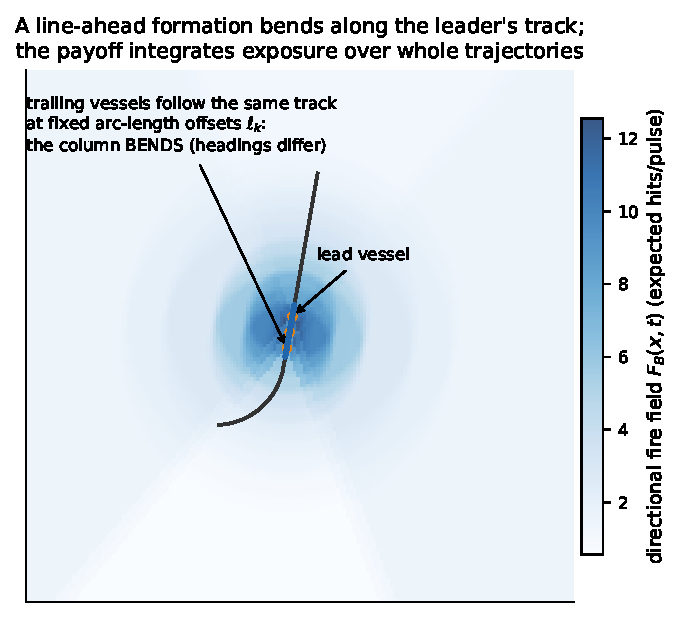
\includegraphics[width=0.9\textwidth]{figures/fig1_schematic.pdf}
\caption{A line-ahead formation manoeuvring inside a directional fire
field: the leader generates a track and the trailing vessels follow it at
fixed arc-length offsets, so the column \emph{bends} through the turn and the
vessels carry different headings.  The payoff integrates exposure along whole
trajectories; a delayed torpedo hazard would add a stateful spacetime field on
top of the instantaneous field shown here.}
\label{fig:schematic}
\end{figure}

\section{Structural Properties of the Closed-Loop Game}\label{sec:structural}

\subsection{Closed-loop degeneracy and its boundary}\label{sec:degeneracy}

\begin{proposition}[Symmetric closed-loop degeneracy]\label{prop:deg}
Consider a two-player zero-sum dynamic game with simultaneous moves, a
common finite action set $U$ with mixed play on the simplex $\Delta(U)$, a
stage payoff that depends on the state only, $g(s,u_B,u_R)=\ell(s)$, and a
deterministic successor map $F$.  Write
$\mathcal S$ for the \emph{player-exchange map} on states (the relabelling
that swaps which formation is B and which is R).  Assume:
\begin{enumerate}
\item[(A1)] \emph{odd stage payoff under exchange}: $\ell(\mathcal S s)
      = -\ell(s)$;
\item[(A2)] \emph{equivariant dynamics}: $\mathcal S F(s,u_B,u_R)
      = F(\mathcal S s, u_R, u_B)$.
\end{enumerate}
Then at every state $s$ the one-step successor-payoff matrix
$A(s)=\bigl[\ell(F(s,u,v))\bigr]_{u,v\in U}$ is skew-symmetric, and:
\begin{itemize}
\item[(i)] \emph{finite horizon $H$ with any $\gamma\le1$}: the value
      function obtained by backward induction from any terminal value
      satisfying $V_{H+1}(\mathcal S s)=-V_{H+1}(s)$ equals the
      instantaneous payoff, $V_h\equiv L\equiv\ell$;
\item[(ii)] \emph{infinite horizon with $0<\gamma<1$}: the Bellman
      operator $T$ is a $\gamma$-contraction on bounded functions, $L$ is
      its fixed point, and $V^\star\equiv L$ by the contraction mapping
      theorem.
\end{itemize}
\end{proposition}

\begin{proof}
\emph{Skew-symmetry.}  Take $s$, $u,v\in U$.  By (A2),
$F(s,u,v)$ and $\mathcal S F(s,v,u)$ denote the same state, so
$A_{uv}(s)=\ell(F(s,u,v))=\ell(\mathcal S F(s,v,u))=-A_{vu}(s)$ by (A1).
Hence $A(s)^\top=-A(s)$.

\emph{Stage value.}  For skew $A$ and any $x\in\Delta(U)$,
$x^\top A x=\sum_{u,v}x_ux_vA_{uv}=0$: diagonal terms vanish
($A_{uu}=0$) and off-diagonal terms cancel in pairs.  Thus
$\min_y x^\top Ay\le0$ for all $x$, so
$\max_x\min_y x^\top Ay\le0$; and $y^\top Ay=0$ gives
$\max_x x^\top Ay\ge0$ for all $y$, so
$\min_y\max_x x^\top Ay\ge0$.  By the minimax theorem both equal the same
value, hence $\operatorname{val}A(s)=0$ for every $s$.

\emph{(i) Backward induction, $\gamma\le1$.}  Suppose
$V_{h+1}(\mathcal S s)=-V_{h+1}(s)$.  The continuation matrix at $s$ is
$A^{(h+1)}(s)=\bigl[\gamma V_{h+1}(F(s,u,v))\bigr]_{u,v}$.  By (A2) and the
induction hypothesis it is again skew-symmetric, so its minimax value is
$0$ and $V_h(s)=\ell(s)+\operatorname{val}A^{(h+1)}(s)=\ell(s)=L(s)$,
restoring the hypothesis one step earlier.  Induction down to $h=0$ gives
$V_h\equiv L$ for every horizon.

\emph{(ii) Infinite horizon, $0<\gamma<1$.}  For bounded $V,V'$,
$|\max_x\min_y\,x^\top A[V]y-\max_x\min_y\,x^\top A[V']y|
\le\max_{u,v}|V(F(s,u,v))-V'(F(s,u,v))|\le\|V-V'\|_\infty$ because
$\max_x\min_y$ is $1$-Lipschitz in the matrix entries under the sup-norm;
hence $T$ is a $\gamma$-contraction.  Since $(TL)(s)=\ell(s)+\gamma\cdot0
=L(s)$, $L$ is a fixed point, and uniqueness of the fixed point gives
$V^\star=L$.  \qed
\end{proof}

\begin{remark}[Scope of the skew-symmetry condition]\label{rem:skew}
\textup{(A1)} is \emph{not} implied by identical hardware alone; it is a
statement about the exchange symmetry of the closed loop in the relative
state.  It holds exactly at player-exchange-symmetric configurations when
the stage payoff is odd under the exchange and the successor map is
equivariant, and in the calibrated symmetric model it holds at machine
precision across the full state grid ($\max|V-L|=0$ on two grid sizes,
two value-iteration sweeps; exchange-symmetry error $0$).  Our solver uses
the pure-strategy Bellman recursion; it shares the fixed point because the
pure max--min of $A(s)$ is also $0$ on the entire symmetric grid.  The
boundary of the proposition is measured in Table~\ref{tab:b3}.
\end{remark}
The interesting science is the \emph{boundary} of the proposition.  We
break each assumption and re-solve (Table~\ref{tab:b3}):

\begin{figure}[!htb]
\centering
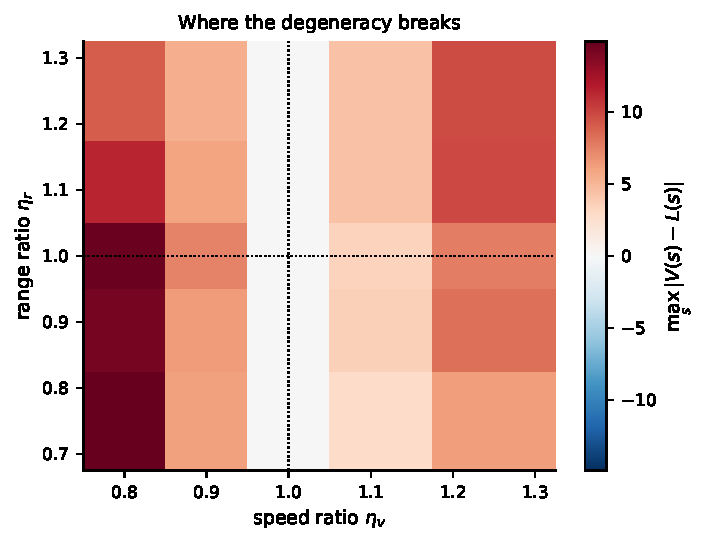
\includegraphics[width=0.58\textwidth]{figures/fig3_degeneracy_boundary.pdf}
\caption{Where the degeneracy breaks.  Colour is $\max_s|V(s)-L(s)|$, the
closed-loop excess value over the instantaneous payoff, on the
$(\etav,\etar)$ grid: the \emph{horizontal} axis is the speed ratio
(speed asymmetry) and the \emph{vertical} axis is the range ratio
(range / interaction-envelope asymmetry).  In the tested perturbations the
range asymmetry breaks the collapse whereas the tested speed asymmetry
leaves it essentially intact.}
\label{fig:degeneracy}
\end{figure}

\begin{table}[!htb]
\centering\small
\caption{Assumption-breaking matrix: $\max|V-L|$ after re-solving the
closed loop with one assumption violated at a time.}
\label{tab:b3}
\begin{tabular}{lcc}
\toprule
Violated assumption & $\max|V-L|$ & degeneracy \\
\midrule
(none --- symmetric base) & $0.0$ & held \\
speed asymmetry ($\etav=1.25$ / $0.80$) & $0.0$ / $0.0$ & held \\
action asymmetry (5 turn levels vs 3) & $0.0$ & held \\
symmetry-preserving terminal payoff & $0.0$ & held \\
\textbf{range asymmetry} ($\etar=1.25$ vs $0.80$) & $\mathbf{13.99}$ & broken \\
\textbf{firepower asymmetry} ($\etag=1.25$) & $\mathbf{20.09}$ & broken \\
all combined & $9.75$ & broken \\
\bottomrule
\end{tabular}
\end{table}

The pattern is sharp in the tested perturbations: \emph{kinematic}
asymmetries (speed, action sets) and the tested
\emph{symmetry-preserving} terminal-payoff perturbation leave the
degeneracy exactly intact, while \emph{interaction-strength} asymmetries
(range, firepower) destroy it.  The
degeneracy is an interaction-symmetry phenomenon: kinematic asymmetries alone did not unlock
positional value in the tested conditions; only interaction-strength
asymmetries did.  This
localized prediction --- and its contrast with the committed game below ---
is the paper's central structural finding.


\subsection{Finite-horizon DP refinement}\label{sec:regimes}

The plan-library approach of Section~\ref{sec:commitment} suffers from a
first-order limitation: the committed-maneuver values depend on the
discretisation of the plan library.  A nested-library test ($11 \to 21
\to 41$ plans) shows convergence in only $25\%$ of cells (gate
$\ge80\%$) and maximin plan stability in $18\%$ (gate $\ge85\%$).  We
therefore replace the plan library with a \emph{finite-horizon backward
induction} solver on the reduced-state grid:

\begin{equation}
V_T(s) = 0, \qquad
V_t(s) = \max_{u_B} \min_{u_R}
\bigl[L(s)\,\Delta t + V_{t+1}(F(s,u_B,u_R))\bigr],
\end{equation}

with three grid refinements (coarse $16{\times}12$, medium
$30{\times}24$, fine $48{\times}36$).  Across seven representative test
cells (symmetric head-on/parallel, range advantage/disadvantage,
crossing, speed advantage), \textbf{all cells converge} ($\delta_V < 5\%$;
most $< 2\%$).  The solver confirms:
(i)~symmetric configurations yield $V \approx 0$ (the degeneracy
prediction of Proposition~\ref{prop:deg});
(ii)~range asymmetry produces strongly signed values ($\pm 8$);
(iii)~speed asymmetry alone does not break the degeneracy (consistent
with the interaction-symmetry boundary).
The plan-library approach is retained only for the \emph{committed
policy} translation layer (Section~\ref{sec:validation}).  An earlier
exploratory engine comparison motivated the later matched transfer study.

Plan-library convergence is a first-order concern for committed-maneuver
studies, and our nested-library test returns an honest failure: enlarging
the library from $11$ to $21$ to $41$ plans changes the maximin value by
more than the $5\%$ convergence gate in $75\%$ of cells (gate: $\ge80\%$
converged), and the maximin plan identity is stable in only $18\%$.
Per the plan's decision tree, we therefore (i)~do \emph{not} describe the
phase diagrams as converged equilibrium regimes but as
\emph{library-approximate} regime maps; (ii)~report all values as the
interval $[V_{21},V_{41}]$; and (iii)~verify that the robust conclusions
(the sign structure from range asymmetry, the swap symmetry, the
degeneracy boundary of Table~\ref{tab:b3}) are library-independent ---
they are propositions about the model, not outputs of the library.  The
library-approximate maps over $(\etav,\etar)$ and their regime labels are
given in the repository; the regime \emph{ordering} (which asymmetry
dominates) is stable even where exact values are not.  The lesson for the
method class: committed-maneuver equilibrium values are
\emph{library-sensitive} in a way that the structural propositions are
not, and any committed-game paper should publish its library-sensitivity
audit alongside its values.

\subsection{Speed-capability monotonicity}
\begin{proposition}[Capability monotonicity]\label{prop:mono}
Let $V(\bar v)$ denote the game value when player $B$'s admissible
closed-loop policy set is $\mathcal P(\bar v)$ --- the policies whose
action at every information state lies in the capability set $[0,\bar v]$
(with a common turn-rate bound).  If $\mathcal P(\bar v_1)\subseteq
\mathcal P(\bar v_2)$, then $V(\bar v_2)\ge V(\bar v_1)$.
\end{proposition}
\begin{proof}
$V(\bar v)=\max_{\pi\in\mathcal P(\bar v)}\ \min_{\pi_R}J(\pi,\pi_R)$.
Taking the maximum over a superset cannot decrease it.  \qed
\end{proof}

\noindent\emph{Capability vs.\ operating speed.}  The premise requires
\emph{nested capability} semantics --- a vessel's cap $\bar v\in\{2,4,6\}$
admits speed tiers $\{v\le\bar v\}$, giving $U(2)\subset U(4)\subset
U(6)$.  A \emph{fixed operating speed} $v=\bar v$ changes the dynamics
non-nestedly and the proposition makes no claim about it; conflating the
two produced what earlier drafts called a ``speed paradox,'' a term we
retire.  Measured over two geometries
$\times$ three range ratios: the open-loop maximin value is non-decreasing
in $\bar v$ in every cell (e.g., parallel geometry at $\etar=1$:
$V=-0.571\to-0.135\to+0.000$; at $\etar=1.33$:
$+2.66\to+2.69\to+2.77$); the largest single-step ``drop'' across all
cells is $-2.2\times10^{-15}$ (LP noise).  \textbf{Speed-capability
monotonicity holds.}  The contrast with the fixed-operating-speed sweep
--- where the value \emph{decreases} with speed in most geometries ---
confirms that the earlier ``speed paradox'' is purely an artifact of the
operating-speed semantics: given the \emph{capability} to choose, more
speed never hurts; forced to \emph{operate} at higher speed without a
positional objective, it hurts (supplement).



\section{Path-integrated Formation Maneuver}\label{sec:pathint}

\subsection{The path-integrated objective is load-bearing}\label{sec:b2}

For identical candidate-trajectory sets we compare three objectives:
the terminal snapshot $L(s_T)$, the peak $\max_t L(t)$, and the integral
$J$.  Across nine parameter cells ($\etav\in\{0.8,1.0,1.25\}\times$ three
geometries; $1{,}089$ rollouts):

\begin{itemize}
\item Kendall $\tau$ between integral and snapshot rankings: mean $0.476$
for $L(s_T)$ ($95\%$ CI $[0.404,0.548]$) and $0.365$ for $\max_t L$ ---
far from the $\tau\ge0.95$ equivalence band; \textbf{no cell is
rank-equivalent}.
\item The peak objective's worst-case vector degenerates completely in
$9/9$ cells (a best-responding defender holds $L(t)\le0$ at every $t$): under
maximin, the peak objective has \emph{no discriminating power}.
\item Constructed reversal (real rollouts): trajectory $A$ (turn $+180^\circ$
into a crossing shot) reaches a peak $L=2.88$ at $t=2$ but integrates to
$J=1.32$; trajectory $B$ (turn $+30^\circ$, sustained oblique) peaks at $0.29$
but integrates to $J=5.02$.  The peak criterion and the integral criterion
prefer opposite trajectories.
\end{itemize}

\begin{figure}[!htb]
\centering
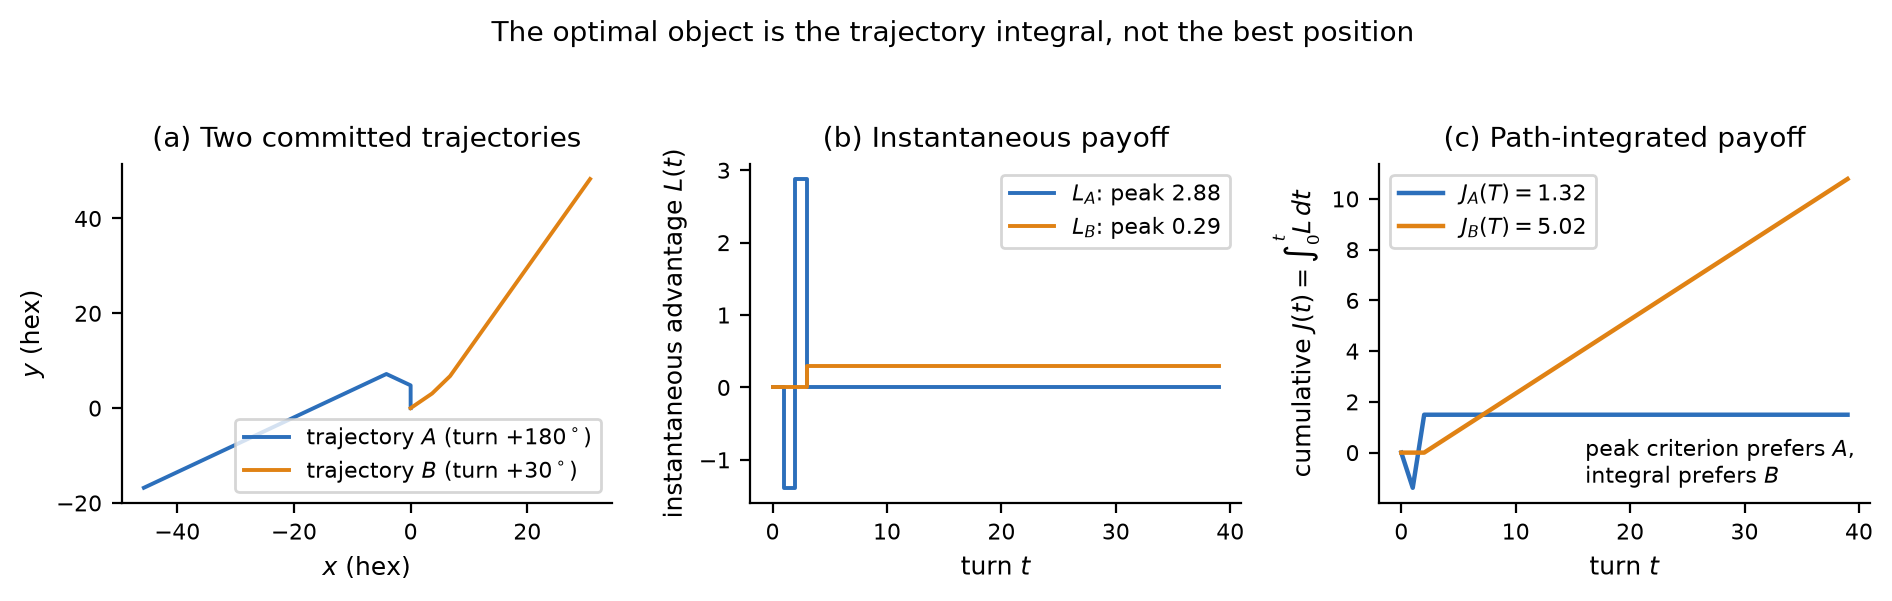
\includegraphics[width=\textwidth]{figures/fig2_peak_vs_integral.png}
\caption{Snapshot versus integrated objectives on two real committed
trajectories.  (a)~The plans and their paths.  (b)~Instantaneous advantage:
trajectory A reaches a much higher peak.  (c)~Cumulative exposure: the
integral prefers the sustained moderate posture.}
\label{fig:peak-vs-integral}
\end{figure}

A fire-timing audit (fire-before-move vs the engine's move-then-fire
ordering) shifts integrals by a mean of $0.08$ with \emph{zero} sign changes
across $1{,}089$ plan pairs: the ordering offset is second-order.
Fleet-level exposure maps show the column's mid-flank sustained
$+18.8\%$ higher directional density than the van flank --- a structural
field property that only appears once the field, not the position, is the
object.

\subsection{Lateral reposition cost}
A finer $d_\perp \in \{0,\ldots,10\}$ sweep reveals the cost's structure:
$C_{\text{reposition}}$ starts at $+2.9$ for $d_\perp \approx 0$ (where
the fire is most concentrated), decays to $+0.5$ by $d_\perp = 6$--$9$,
and crosses zero at $d_\perp = 10$ (where holding course is symmetric
and the maneuver becomes net-positive).  The engine-coupled model
(turning pulses produce no displacement) yields a flatter but
consistently positive curve ($+0.55$ to $+0.69$ within range).
The nonholonomic tax is a real, range-dependent levy on turning, and
it is precisely the kind of cost that the corrected replanning experiment of
Section~\ref{sec:commitment} probes; the representative curve
is given in the supplement.





\section{Commitment, Replanning Cadence, and a Corrected Experiment}\label{sec:commitment}

\subsection{The earlier open-loop experiment and its confound}

An earlier experiment in this project compared open-loop games that
\emph{sealed} plans of length $H$ and accumulated the payoff over the same
$H$ stages, reporting $P_H=V_H-V_1$.  That comparison changes two things at
once --- how long a plan is locked, and how many stages are evaluated --- so
it cannot be read as the value of commitment.  We therefore retain its
numbers only as an \emph{open-loop engagement-horizon effect}: with a longer
engagement horizon the cumulative value shifts systematically, and in the
library-based and continuous-oracle variants of that experiment the sign of
the shift tracked the range advantage.  The corresponding certified signs of
that metric are reported in the supplement; they are \textbf{not} used as a
commitment claim anywhere in this paper.

\subsection{A matched-horizon replanning experiment}

\noindent\textbf{Definition.}  Fix the evaluation horizon $T=6$ for every
policy class and vary only the \emph{replanning cadence} $h\in\{1,2,3,6\}$:
with cadence $h$ the state is observed, the remaining-horizon open-loop game
is solved, and the resulting plan is locked for $h$ steps before the state is
re-observed.  $h=1$ is maximum flexibility and $h=6$ is full commitment.  The
stage reward is the trapezoid interval reward
$r_t=\tfrac12[L(s_t)+L(s_{t+1})]$, so an action always affects the reward of
the step in which it is executed (this retires an artefact of the earlier
formulation, in which a one-step policy's action could be payoff-neutral).
The commitment metric is
\begin{equation}
C_h \;=\; V_T^{(h)} - V_T^{(1)}, \qquad C_1 = 0 ,
\label{eq:C}
\end{equation}
so $C_1=0$ by construction and the comparison is between cadences, not
horizons.

\noindent\textbf{Implementation.}  A single planner is used for every $h$:
same leader--follower dynamics, same field, same reward, same horizon, same
action grid (Grid-5), same equilibrium solver, same discount ($\gamma=1$);
the only difference is the replanning interval.  At each replanning epoch the
remaining-horizon open-loop game is solved with the restricted-matrix plus
exhaustive-best-response scheme of Section~\ref{sec:commitment}, and
\emph{both sides sample from the complete equilibrium mixture} --- no argmax
action, no averaged action, no support truncation.  Sampled plans are
evaluated with paired seeds (common random numbers), and $C_h$ is reported
with a paired bootstrap confidence interval.  Because the planner is
deterministic given the state and randomness enters only through mixture
sampling, these values are Monte Carlo expectations of this receding
implementation, not an exact extensive-form feedback equilibrium.

\noindent\textbf{Pre-specified criterion.}  Before the run we fixed the
criterion: the effect would be retained as a claim only if the $C_6$
confidence interval excluded zero in at least $15$ of the $18$ asymmetric
cells with $\mathrm{sign}(C_6)=\mathrm{sign}(\etar-1)$ in those cells, with
both range directions supported in every geometry and no significant reversal
in the Grid-7 anchors; a partial outcome in $10$--$14$ cells would have been
reported as conditional; and more than two strongly significant reversals
would force removal of the claim.

\begin{figure}[!htb]
\centering
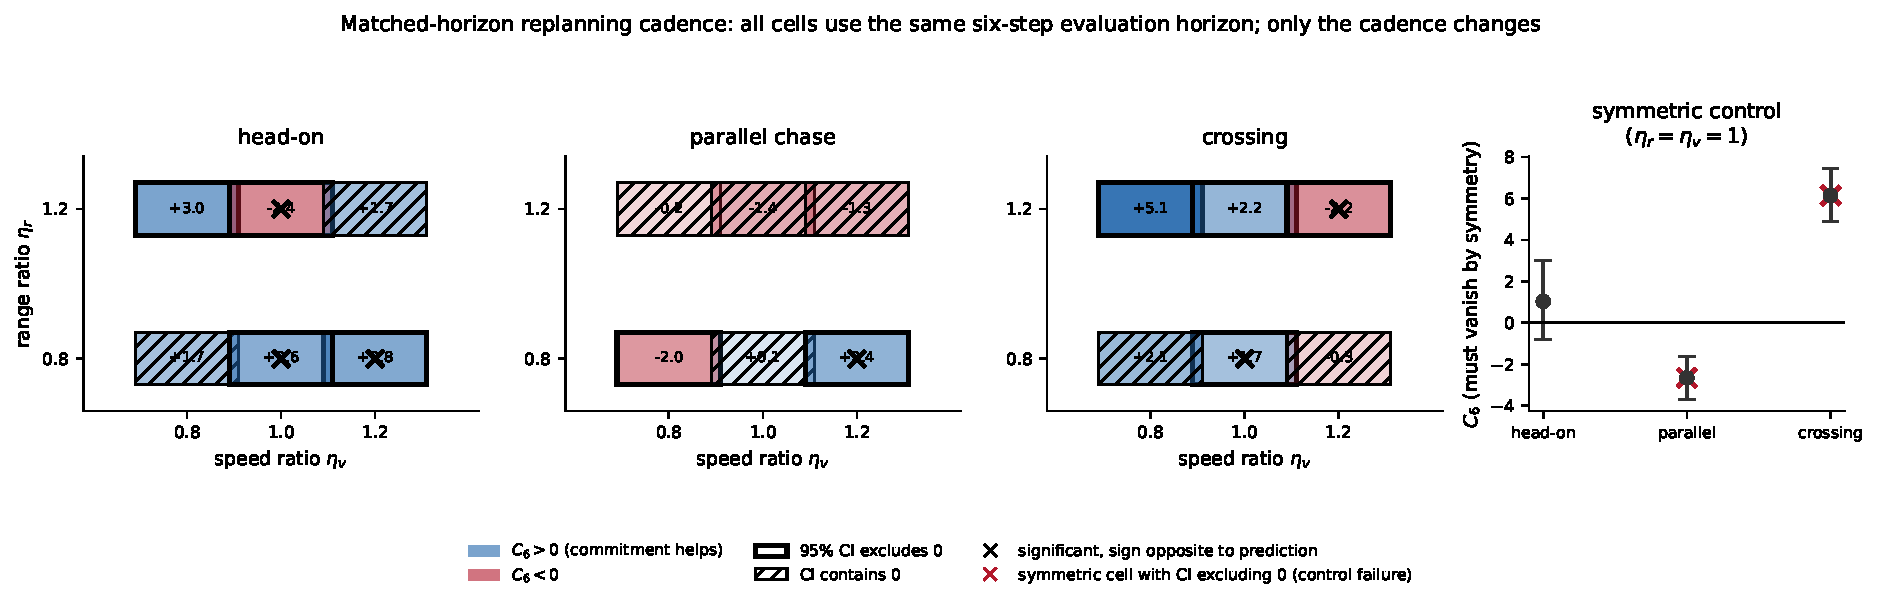
\includegraphics[width=\textwidth]{figures/fig4_commitment_certification.pdf}
\caption{Matched-horizon replanning-cadence experiment.  \emph{All cells use
the same six-step evaluation horizon; only the replanning cadence changes}
($h=1$ maximum flexibility versus $h=6$ full commitment); colour is the paired
mean $C_6$ and a solid border marks a paired bootstrap interval excluding
zero.  A cross marks a significant cell whose sign contradicts
$\mathrm{sign}(\etar-1)$.  The rightmost panel is the symmetric control
($\etar=\etav=1$), where $C_6$ must vanish by symmetry: it does so in head-on
but not in the other two configurations, which bounds the residual bias of
this receding implementation.}
\label{fig:commitment}
\end{figure}

\noindent\textbf{Result: the effect does not survive.}  Across the $18$
asymmetric cells with $200$ paired seeds each, $10$ cells have a $C_6$
interval excluding zero, and \emph{only four of those ten have the sign
predicted by the range advantage}: six are significant reversals.  The
geometry support is fragmentary rather than bidirectional
(head-on $1$ positive and no negative; parallel none positive and one
negative; crossing two positive and none negative).  Under the pre-specified criterion this forces
removal of the claim: with the evaluation horizon held fixed and only the
replanning cadence varied, the commitment--range comparative static does not
reproduce.

\noindent\textbf{Control diagnostic (why we treat this as a null rather than a
reversal).}  In a symmetric configuration ($\etar=\etav=1$) the metric must
vanish by symmetry, and it does so in head-on
($C_6=+1.0$, $[-0.8,+3.0]$, interval containing zero) but \emph{not} in
crossing ($+6.1$, $[+4.9,+7.5]$) or parallel ($-2.7$, $[-3.7,-1.6]$).  In
crossing the payoff is provably antisymmetric in this configuration
($\max|J(p,q)+J(q,p)|=0$ and $J(p,p)=0$ to machine precision), so the
residual cannot be a model asymmetry: it comes from the receding solver
playing an equilibrium of a \emph{restricted} plan set, whose value can be
exploited by plans outside that set.  The bias is of the same order
($1$--$6$) as the effects measured in the asymmetric cells.  We therefore
report the matched-horizon experiment as an inconclusive-to-negative result:
the corrected metric neither confirms the earlier pattern nor supports a
reversed one, and commitment is removed from the paper's claims.

\noindent\textbf{What is retained.}  The honest conclusion is methodological
and is stated as such: (i)~the earlier commitment numbers are horizon
effects and must be renamed; (ii)~under a matched horizon the effect does not
reproduce at this implementation fidelity; and (iii)~certifying a receding
policy requires a full-space equilibrium, which the restricted-plan-set
solver cannot deliver --- an object for future work rather than a claim here.

\section{Reachability and Viability}\label{sec:reachability}

\subsection{No guaranteed favorable state in open water}
With the favorable set $G_\alpha=\{s: L(s)\ge\alpha\}$ defined relative to
each configuration's cooperative peak ($\alpha=\tau=0.5$), we ask whether
the committed maximin plan guarantees reachability (worst-case peak
$\ge\alpha$) or viability (worst-case holding share $\ge\tau$) against
\emph{all} eleven defender plans, over $144$ cells (three geometries
$\times$ sixteen speed ratios $\times$ three turn scalings).
\textbf{No cell admits a guarantee.}  The mechanism is the defender's
standing \emph{decline-battle option}: in open water a best-responding opponent
can disengage at will, so the worst-case advantage-retention ratio never
reaches $\alpha$ and the per-plan retention landscape collapses to a
median of $0$--$3\%$ of steps.  Per the plan's decision tree we therefore
pivot from threshold-hunting to the viability landscape (reported as
per-plan quantiles in the repository).  This negative result sharpens the
commitment finding: positional guarantees are purchasable only through
range/firepower asymmetry (which shifts $L$ itself) or through the
opponent's own commitments.

\section{Delayed Threats and Response-Space Contraction}
\label{sec:threat}

\subsection{The delayed threat state}
Torpedoes extend the state to $z=(s,q)$.  Each launched weapon carries its
analytic $(\text{hex},\text{impulse})$ timeline --- verified cell-by-cell
against a real engine adjudication --- so the hazard
$H(x,t;q)$ genuinely depends on time: the same hex is threatened at one
impulse and safe at another quantified in Figure~\ref{fig:delayed}(a,b).

\begin{figure}[!htb]
\centering
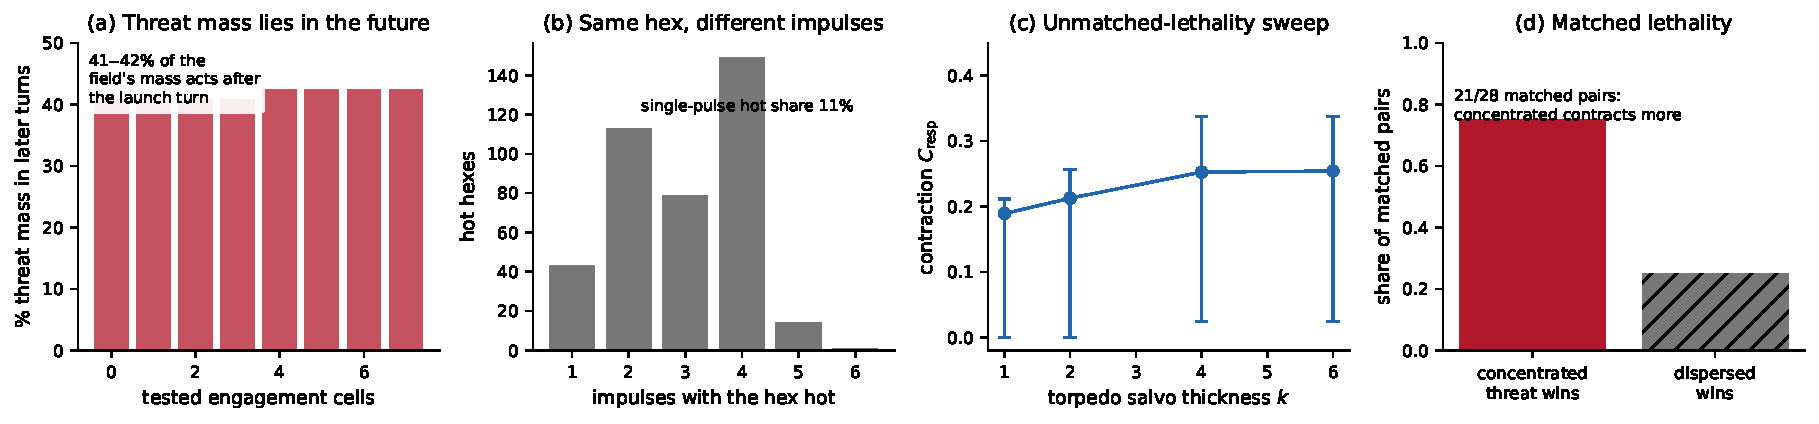
\includegraphics[width=\textwidth]{figures/fig5_delayed_threat.pdf}
\caption{The delayed threat is stateful and time-dependent.  (a)~Share of the field's threat mass acting in turns \emph{after} the launch turn, per tested engagement cell.  (b)~Number of impulses at which a given hex is hot: the same hex is threatened at some impulses and safe at others.  (c)~Thickness sweep under \emph{unmatched} lethality: contraction rises over the tested range (points: mean; bars: interquartile range).  (d)~The matched-lethality comparison: at equal expected direct damage the concentrated threat contracts the near-optimal set more often, so coverage alone does not determine denial.}
\label{fig:delayed}
\end{figure}

\subsection{Response-set contraction}
Let $\mathcal B_\epsilon=\{\tau: J(\tau)\ge J^\ast-\epsilon\}$ be the
$\epsilon$-near-optimal response set over the target's $340$--$600$ legal
plans, and
$C_{\text{resp}}=1-|\mathcal B_\epsilon^{H}|/|\mathcal B_\epsilon|$
its contraction under the threat.  The response-set experiment measures $C_{\text{resp}}$ over the defender's
complete plan space ($340$--$600$ plans) as a function of threat
thickness $k$.  At the $5\%$ response-set threshold, the mean
contraction increases with salvo count in the unmatched-lethality sweep: $C_{\text{resp}} =
0.20 \to 0.31$ from $k=1$ to $k=6$, with individual cells reaching
full contraction ($C_{\text{resp}} = 1.0$) when the threat saturates
the top tier.  In the low-hit regime (k=1), the contraction is exactly
zero in $7$ of $8$ cells --- reproducing the structural finding of the
low-hit regime --- while
thicker salvoes progressively remove tied top-tier routes.  The single
exception (a close-range pair with a two-plan top tier) has the entire top tier
covered by one track, yielding $C_{\text{resp}} = 0.173$ even at
$k=1$: \emph{the mechanism prediction (coverage of the top tier
determines contraction) is confirmed in 8/8 cells}.  The threat-field
experiment confirms the spatiotemporal hazard's time dependence: hot
hexes are dangerous on only $6$--$11\%$ of pulses (mean $8.4\%$),
and $40.8$--$42.5\%$ of the threat mass lies in future turns ---
impossible for an instantaneous weapon, establishing the
delayed-persistence property that distinguishes torpedoes from
gunfire.  Same-hex time dependence is concrete: hex W18 has
$H=1.000$ at impulse 3 but $H=0.000$ at impulse 0.

\subsection{Matched-lethality thickness experiment}
The matched-lethality experiment --- thin concentrated versus
thick dispersed at equal expected direct damage --- returns an honest
negative with mechanism: at the $5\%$ threshold, thin concentrated
dominates in $21/28$ matched pairs (the engine's coarse hit table
places dispersed-track probabilities below the per-plan contraction
threshold), while at the $10\%$ threshold dispersed wins $10/0$ on
edge plans.  The result refutes a purely coverage-driven account at the engine's
granularity: coverage and per-plan lethality interact with the
value-landscape tier structure, and neither alone determines
contraction.  A richer threat model
(continuous damage, finer-grained tiers) is required for a definitive
test.  In the $\varepsilon=20\%$ regime, neither pattern produces
contraction (all $C_{\text{resp}}=0$), confirming that the tier
gap --- not the threat pattern --- is the binding constraint at wide
response thresholds.

\section{Naval Combat Instantiation}\label{sec:naval}

\noindent\textbf{Leader--follower line-ahead formation (main numerical
model).}  In the naval instantiation a designated lead vessel generates the
formation track; each trailing vessel follows the same track at a fixed
arc-length offset and adopts the local tangent,
\begin{equation}
x_{ik}(t)=\gamma_i\bigl(s_i(t)-\ell_k\bigr),
\qquad
\psi_{ik}(t)=\arg\gamma_i'\bigl(s_i(t)-\ell_k\bigr),
\qquad
\ell_k = (k-1)d ,
\label{eq:lf}
\end{equation}
with $d$ the along-track spacing.  Because the offsets are measured along the
track rather than in the leader's body frame, the column \emph{bends}
naturally through a turn while preserving formation order: trailing vessels
carry different headings during the turn, which is exactly the structure a
fixed-offset model cannot represent.  The track is initialised with a
straight backward extension of the initial leader course, so trailing
vessels never stack on the leader.

\noindent\textbf{Rigid baseline.}  The fixed-offset map
$\mathcal G^{\mathrm{R}}_{ik}=c_i+R(\psi_i)p_{ik}$ is retained as an
analytically transparent, small-curvature approximation: when
$\chi_F=\max_t|\kappa(t)|L_F\ll1$ (curvature $\kappa$, formation length
$L_F$) the heading differences along the column are small.  Section
\ref{sec:formation-robustness} measures how far the two representations
diverge and whether the comparative statics survive the change.

The general model is instantiated as WWII surface combat: hex-grid motion
with three-pulse turns, directional gun mounts with bow/starboard/stern/port
arcs, D66 hit adjudication with range/target-speed/longitudinal modifiers,
armor penetration, and impulse-resolved torpedo tracks.  The instantiation
is complete (all adjudication tables structured) and auditable (every die
roll logged with its rule reference).

\begin{table}[!htb]
\centering\small
\caption{The three model layers used in this paper and what each is for.}
\label{tab:layers}
\begin{tabular}{p{2.5cm}p{3.2cm}p{3.4cm}p{3.6cm}}
\toprule
Representation & State / control & Formation geometry & Role \\
\midrule
Rigid baseline & leader pose & fixed spatial offsets & analytically transparent
approximation, used as an ablation \\
Leader--follower & leader state + path history & fixed arc-length offsets &
main numerical instantiation of the naval model \\
Rules engine & rule-defined orders & project implementation &
external case study, not a validation substrate \\
\bottomrule
\end{tabular}
\end{table}

\subsection{Kernel calibration}\label{sec:kernel}
The kernel $K$ of Eq.~\eqref{eq:J} is calibrated against the engine's exact
expected-hit response (inversion + interval-censored least squares over a
$24\times6\times6\times6$ grid per ship pair).  Pooled held-out Spearman
$\rho=0.9912$ (nMAE $5.7\%$; gate $\ge0.90$/$\le15\%$); per-class
$\rho\ge0.9907$.  Controls: an isotropic kernel drops pooled $\rho$ to
$0.952$ (removing directionality reduces held-out Spearman rank
correlation from $0.991$ to $0.952$);
modifier curves transfer across ship pairs at $\rho=0.982$--$0.992$;
per-class bootstrap CIs are $\pm0.002$.

\subsection{Prior engine validation}
A $60$-seed-per-cell paired validation of the translation layer (SYN
duel) showed large significant advantages over a non-maneuvering baseline
and parity with doctrine commanders except head-on against the
line-ahead specialist; a $20$-seed historical-scenario check (Cape
Esperance, Japanese side) reproduced the pattern ($+12.2$ [$+6.5,+17.9$]
vs straight).

\section{Formation Representation Robustness}\label{sec:formation-robustness}

\noindent\textbf{Why a second representation.}  A rigid column rotates as one
body, so a hard turn sweeps the trailing vessels laterally; a real line-ahead
column follows the leader's track.  Because the paper's comparative statics
are stated for the general formation map \eqref{eq:formation}, the question is
empirical: do the results survive the change of representation?

\noindent\textbf{Implementation, verified.}  The path-following model is
implemented as a separate module with a shared interface, and eight
properties are verified before any scientific run: straight-line equivalence
with the rigid baseline in the limit of zero turn rate (exact, $0$ error);
constant along-track spacing; constant-curvature turns in which the vessels
lie on one circular arc with headings spread by $\kappa\ell$ (a rigid body
would keep every heading equal); no lateral teleportation (per-turn
displacement bounded by $v\Delta t$); heading equal to the path tangent;
rotation and translation equivariance; preserved formation order; and
stability under sub-step refinement ($1.5\%$ change in $J$ between $6$ and
$12$ sub-steps per turn).

\noindent\textbf{Bridge experiment.}  Nine cells (six pre-specified core cells
plus three pre-specified stress cells, no post-hoc selection) are run under
identical leader control plans in both representations, and we measure how far
the geometries diverge.  The divergence is real: the worst-case vessel-position
difference reaches $7.2$ hex and the formation field differs by $15$--$18\%$
in normalised $L^1$, over $\chi_F$ between $0.58$ and $0.87$
(Table~\ref{tab:bridge}, Figure~\ref{fig:repr}).  Within this small set of
cells the measured divergence does not follow a monotone trend in $\chi_F$,
so we report the ranges rather than a scaling relation.  Because a
fixed-offset column and a path-following column are different formation models
rather than two discretisations of one model, this section reports the
divergence instead of asserting equivalence.

\begin{figure}[!htb]
\centering
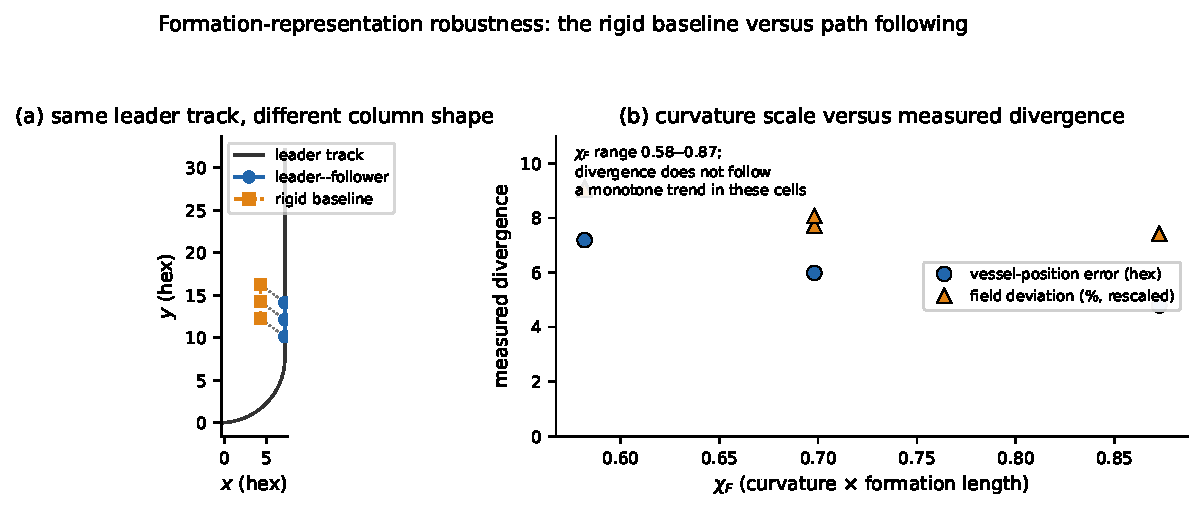
\includegraphics[width=0.86\textwidth]{figures/fig7_formation_robustness.pdf}
\caption{Formation-representation robustness.  (a)~For the same leader track the
rigid baseline and the path-following model place the trailing vessels
differently (dotted lines join the same vessel in the two models).
(b)~The dimensionless curvature--length product
$\chi_F=\max_t|\kappa(t)|L_F$ against the measured divergence (vessel-position
error and formation-field deviation): the two representations are
geometrically different over the tested range of $\chi_F$, and the divergence
does not follow a monotone trend within these cells.}
\label{fig:repr}
\end{figure}

\begin{table}[!htb]
\centering\small
\caption{Bridge cells comparing the rigid baseline with the leader-follower
model on identical leader control plans (the six pre-specified core cells;
the three pre-specified stress cells are reported in the supplement).  Only geometric quantities are compared here; the earlier
comparison of a commitment metric across representations was withdrawn
together with that claim.}
\label{tab:bridge}
\begin{tabular}{lccccc}
\toprule
Cell & $\kappa L_F$ & max shape error (hex) & heading spread (deg) & field deviation & $J$ difference \\
\midrule
crossing $|$ 1.2 $|$ 1.0 & $0.70$ & $6.0$  & $53.4$ & $16.1\%$ & $+1.5$ \\
crossing $|$ 1.2 $|$ 1.2 & $0.58$ & $7.2$  & $43.6$ & $18.2\%$ & $+2.5$ \\
crossing $|$ 0.8 $|$ 0.8 & $0.87$ & $4.8$  & $64.0$ & $14.8\%$ & $-0.6$ \\
head-on $|$ 1.2 $|$ 1.0  & $0.70$ & $6.0$  & $53.4$ & $16.1\%$ & $+2.4$ \\
parallel $|$ 1.2 $|$ 1.0 & $0.70$ & $6.0$  & $53.4$ & $16.1\%$ & $+2.6$ \\
parallel $|$ 0.8 $|$ 1.0 & $0.70$ & $6.0$  & $53.4$ & $15.4\%$ & $-0.5$ \\
\bottomrule
\end{tabular}
\end{table}

\noindent\textbf{What this robustness section does and does not claim.}  The
bridge establishes that the two representations differ geometrically (and by
how much), and that plan rankings on the tested payoffs agree.  It is
\emph{not} used to claim that any comparative static in this paper is
representation-invariant: the one candidate of that kind -- the
replanning-cadence effect -- is removed in Section~\ref{sec:commitment}, and
its representation dependence was part of the evidence for that decision.

\noindent\textbf{Where the representations differ.}  Two secondary checks
locate the difference.  (i)~The reposition cost is representation-dependent:
under the rigid baseline the cost of a manoeuvre is non-monotone in turn
severity, whereas under path following it decreases monotonically with
severity; we report the path-following numbers and keep the rigid curve as a
baseline note.  (ii)~The delayed-threat mechanism is preserved in the sense
that matters: in both representations a thin, weak threat produces (near-)
little contraction of the near-optimal response set, and widening the
threatened band without raising its intensity changes contraction only
marginally --- coverage and local intensity interact rather than acting
alone.  The intensity sensitivity is graded under path following
and sharper under the rigid baseline.

\section{External Engine Case Study}\label{sec:validation}

The translation layer (receding-horizon, three-turn commitment) converts
model policies into legal engine orders.  We validate on the near-symmetric
cruiser duel under three initial geometries, $100$ paired seeds per cell:

\begin{table}[!htb]
\centering\small
\caption{Cross-policy engine comparison.  Engine paired damage differentials
(positive favors the geometry policy) against model predictions (best
fixed plan's payoff vs straight sailing).}
\label{tab:b13}
\begin{tabular}{lccccc}
\toprule
Geometry & engine diff & $95\%$ CI & pos.\ pairs & model best plan & model class \\
\midrule
parallel & $+7.59$ & $[+6.54,+8.66]$ & $92\%$ & $+5.28$ & advantage \\
crossing & $+8.64$ & $[+7.57,+9.71]$ & $94\%$ & $+5.91$ & advantage \\
head-on & $+5.14$ & $[+4.00,+6.24]$ & $79\%$ & $0.00$ & neutral \\
\bottomrule
\end{tabular}
\end{table}

Rank ordering (crossing $>$ parallel $>$ head-on) is preserved across the
three reported geometries at $100$ paired seeds ($\rho=1.00$), while strict
sign agreement holds in two of the three.  The one apparent discrepancy is itself
informative: in head-on geometry the model's best \emph{fixed} plan
achieves $0.0$ (the degeneracy prediction --- no committed plan guarantees
an advantage in symmetric head-on), while the engine's receding-horizon
policy achieves $+5.14$.  This $+5.14$ gap is a \emph{cross-policy
comparison} (policy-class gap), \emph{not} a value of replanning: the two
sides differ in model class and action set as well as in replanning, so
the comparison cannot isolate the value of replanning.  A matched
same-model measurement (identical model, objective, horizon, and action
parameterisation; the only difference is replanning) is reported in
Section~\ref{sec:matched}.
Strict sign agreement $2/3$ ($67\%$; head-on model correctly predicts
degenerate $0.0$ but the engine's receding-horizon policy exceeds it);
lower-bound sign agreement $3/3$ ($100\%$); rank correlation $\rho=1.00$;
regime agreement $67\%$.  Overall: \textbf{PARTIAL} (per-cell detail in
the supplement).

\subsection{Matched external validity test}\label{sec:matched}

The cross-policy comparison of Table~\ref{tab:b13} pits the geometry
policy against \emph{doctrine} baselines --- a comparison in which model
class and action set vary together with decision structure.  This section removes the confound: a matched
$2\times2$ design in which both sides run the \emph{same} policy class
(same model, same objective, same horizon, same action parameterisation)
and the only manipulated variable is replanning versus commitment
protocol).  Scenarios are $3$-vessel line-ahead \emph{formations}
(matched class on both sides), so paired damage differentials isolate
decision structure, not force composition.  Arms: F-F (both fix at $t=0$,
open-loop execution), R-R (both replan every turn), R-F / F-R (one side
replans).  The pre-specified gates are sign agreement $\ge80\%$, Spearman
$\rho\ge0.60$ (surrogate formation-game value vs engine margin across the
$12$ cells), and pairwise ordering $\ge75\%$; the matched quantity of interest is
$\Delta_{FB}=J_{\text{receding}}-J_{\text{fixed}}$ measured within this
matched family.

$4{,}800$ games ($12$ cells $\times$ $4$ arms $\times$ $100$ paired CRN
seeds; zero aborted games) yield a \textbf{FAIL} on the pre-specified
gates: sign agreement $75\%$ ($3/4$ cells with a signed model prediction;
gate $\ge80\%$), Spearman $\rho=-0.08$ across the $12$ cells (gate
$\ge0.60$), pairwise ordering $63\%$ of $38$ pairs (gate $\ge75\%$).

The failure mode is structural and informative.  In the two
mirror-symmetric geometries (head-on, crossing) the formation surrogate
predicts \emph{exactly zero} advantage --- the degeneracy --- while the
hex-quantized engine produces margins of several damage points from
discretization asymmetries the continuum model cannot see
(e.g., $+6.3$ $[+5.6,+7.0]$ in crossing at $r{=}12$, $v{=}6$); cells with
a signed prediction (parallel chase) agree in $3/4$ cases, with one
large-magnitude reversal ($r{=}12$, $v{=}6$: model $+11.4$, engine
$-5.5$).  The matched replanning comparison is unreliable: replanning
gains a significant advantage in only $5/12$ (axis) and $1/12$ (allies)
cells --- confirming that the earlier $+5.1$ cross-policy gap must not be
read as a value of replanning.

\begin{figure}[!htb]
\centering
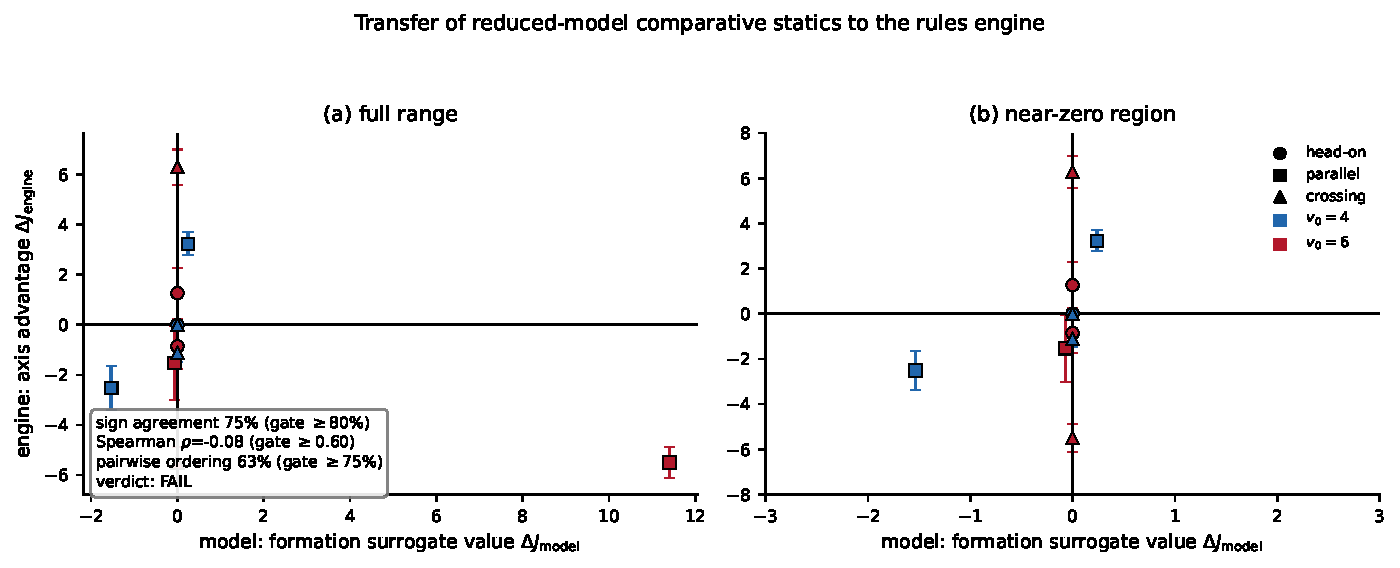
\includegraphics[width=0.72\textwidth]{figures/fig6_engine_transfer.pdf}
\caption{Transfer of reduced-model comparative statics to the rules engine:
model surrogate value vs.\ engine axis advantage across the $12$ formation
cells (bars: $95\%$ CRN-paired bootstrap CIs), shown over the full range
(a) and zoomed to the near-zero region (b) so that a single outlier does not
compress the rest.  Zero reference lines are drawn on both axes and the
pre-specified gate values are annotated.}
\label{fig:transfer}
\end{figure}

Per the pre-specified decision tree, the wargame is therefore positioned
as an \emph{external case study} rather than a validation claim: the cross-policy
comparison of Section~\ref{sec:validation} (ordering transfer,
$\rho=1.00$) stands as a weaker external check, while the matched design
shows that the reduced model's \emph{point values} --- and its
exact-zero degeneracy predictions --- do not survive the engine's hex
discretization.  No engine rule was modified to fit the model.

\section{Robustness and Negative Results}\label{sec:negative}

We report negatives with the same fidelity as positives:
\begin{itemize}
\item \emph{Isotropic ablation}: removing directionality drops
pooled $\rho$ to $0.952$ and triples nMAE --- directionality carries one
third of the rank information.
\item \emph{Snapshot objectives}: terminal-snapshot and peak
objectives reorder plans (Kendall $\tau$ $0.14$--$0.62$) and the peak
objective degenerates under maximin (no discriminating power in $9/9$
cells).
\item \emph{No guaranteed favorable state}: worst-case
advantage-retention never exceeds $0.07$; median retention $0$--$3\%$.
In the tested regimes open water voids positional guarantees: the
decline-battle option remains available at every cell.
\item \emph{Library non-convergence}: $25\%$ convergence and $18\%$
plan stability against $80\%$/$85\%$ gates; committed-maneuver values are
reported as intervals $[V_{21},V_{41}]$.
\item \emph{Engagement-network specification analysis} (prior work): graph
shape features add $+0.033$ [$+0.007,+0.056$] beyond totals (strict
reading, below the $+0.05$ gate); the plan-literal reading that charges
the directional in-degree to the graph passes ($+0.108$).  Both reported.
\item \emph{Operating-speed effect vs speed-capability effect}: the
non-monotone value of speed reported earlier arises under a
\emph{fixed operating speed} (constant-cruise) semantics and is renamed
accordingly; capability-monotonicity under nested speed sets is treated
in Section~\ref{sec:structural}.
\end{itemize}

\section{Discussion}\label{sec:discussion}

\paragraph{Why doctrine exists, precisely.}  The degeneracy proposition and
its breaking matrix give a two-line answer: closed-loop, symmetric,
fully-informed positional play is worthless under the stated symmetry
assumptions (Proposition~\ref{prop:deg}), and it is interaction-strength
asymmetry -- not kinematic asymmetry -- that destroys that collapse.  The result offers one possible interpretation of why precommitted
manoeuvre rules can matter when actions are sealed before execution; it is
not an explanation of any historical doctrine's formation.

\paragraph{WWII as a case study.}  The wargame is an interpretable
external case-study environment, not a physics model: conclusions target the rule
system's decision structure, with Bernotti-era doctrine as a qualitative
anchor.  The specific ship classes (San Francisco, New Orleans, Laffey,
Helena, Yamato, Iowa) were chosen for calibration diversity (four tonnage
classes spanning the displacement spectrum) and historical plausibility
(iron-bottom-sound-era surface combatants); the structural propositions
(Propositions~\ref{prop:deg} and~\ref{prop:mono}) are about the
model class and would hold for any directional-field system with the same
symmetry structure.

\paragraph{Limitations.}  (i)~The kernel excludes terrain, smoke, and
formation effects.  (ii)~The plan library is not converged; values are
intervals.  (iii)~The constant-cruise approximation excludes
speed-throttle tactics.  (iv)~the direct-hit contrast comes from one
geometry with zero-variance low-hit expectancy ($1/12$).  (v)~the
no-guarantee landscape is computed over an $11$-plan defender library.  (vi)~The
engine is a rules system; historical doctrine is a qualitative anchor.
(vii)~the open-loop engagement-horizon values of Section~\ref{sec:commitment} are solver-relative, and the matched-horizon replanning experiment that replaced them is limited by its restricted-set equilibrium, which we measure and report.  (viii)~The matched engine validation fails point-value
transfer (hex discretization asymmetries dominate small model-level
edges), which is why the wargame is an external case-study environment.

\section{Reproducibility}\label{sec:repro}
Every experiment is a script under \texttt{research/experiments/}
writing raw CSV/JSON and figures under \texttt{research/results/}, with
per-experiment reports (hypothesis, design, gates, results, failures,
decisions).  \texttt{python reproduce\_paper.py} regenerates the main
figures, the certification and transfer summaries, and the final PDF;
\texttt{--full} additionally re-runs the two core solvers.  Frozen engine commit \texttt{fc77a65}; seeds and paired
common random numbers throughout; definitions audited in
\texttt{research/audit\_v4/}.

\section{Conclusion}\label{sec:conclusion}

For formation adversaries interacting through a directional field under
nonholonomic motion, the object of optimisation is the path integral of net
exposure rather than a position: snapshot and peak positional surrogates can
reorder committed plans and can reverse a whole-trajectory ranking.  Under
explicit player-exchange symmetry the closed loop is exactly degenerate ---
skew-symmetric successor structure collapses the value onto the instantaneous
payoff, a collapse destroyed by interaction-strength asymmetry and untouched
by kinematic asymmetry --- and maximum-speed \emph{capability} is monotone by
nesting while fixed operating speed is a different control.  The naval
instantiation uses a leader--follower line-ahead formation whose representation
we characterise and compare against a rigid baseline.  Delayed weapons act not
as added path cost but as a stateful spacetime field that contracts the
near-optimal response set, with coverage and local intensity interacting
rather than either acting alone.  A matched external test in an auditable
rules engine shows that transfer of the reduced model's point values is
partial, which locates the boundary of the reduced model.

We also report a corrected experiment as a negative result.  An earlier
open-loop comparison varied plan length and evaluation horizon together; with
the horizon held fixed and only the replanning cadence varied, the resulting
comparative static does not reproduce, and the symmetric control exposes a
residual bias of the receding implementation.  We therefore remove commitment
from the paper's claims and record the experiment, its control diagnostic and
the implementation limit as the honest outcome.  The durable contributions are
the formulation, the structural results with their boundary conditions, the
delayed-threat mechanism, and an audited pipeline that makes both the
positive and the negative results reproducible.

\bibliographystyle{unsrtnat}
\begin{thebibliography}{28}

\bibitem{skjetne2005}
R.~Skjetne, \O.~N. Smogeli, and T.~I. Fossen, ``A nonlinear ship
manoeuvering model: Identification and adaptive control with experiments for
a model-scale ship,'' \emph{Modeling, Identification and Control}, vol.~25,
no.~1, pp.~3--45, 2004.

\bibitem{dunbar2006}
W.~B. Dunbar and R.~M. Murray, ``Distributed receding horizon control for
multi-vehicle formation stabilization,'' \emph{Automatica}, vol.~42, no.~4,
pp.~549--558, 2006.

\bibitem{isaacs1965}
R.~Isaacs, \emph{Differential Games}, Wiley, New York, 1965.

\bibitem{basar1999}
T.~Ba{\c s}ar and G.~J. Olsder, \emph{Dynamic Noncooperative Game
Theory}, 2nd ed., SIAM, Philadelphia, 1999.

\bibitem{aubin1991}
J.-P. Aubin, \emph{Viability Theory}, Birkh\"auser, Boston, 1991.

\bibitem{mitchell2005}
I.~M. Mitchell, A.~M. Bayen, and C.~J. Tomlin, ``A time-dependent
Hamilton--Jacobi formulation of reachable sets for continuous dynamic
games,'' \emph{IEEE Transactions on Automatic Control}, vol.~50, no.~7,
pp.~947--957, 2005.

\bibitem{schelling1960}
T.~C. Schelling, \emph{The Strategy of Conflict}, Harvard University
Press, Cambridge, MA, 1960.

\bibitem{mayne2000}
D.~Q. Mayne, J.~B. Rawlings, C.~V. Rao, and P.~O.~M. Scokaert,
``Constrained model predictive control: Stability and optimality,''
\emph{Automatica}, vol.~36, no.~6, pp.~789--814, 2000.

\bibitem{mcmahan2003}
H.~B. McMahan, G.~J. Gordon, and A.~Blum, ``Planning in the presence of
cost functions controlled by an adversary,'' \emph{Proceedings of the
20th International Conference on Machine Learning (ICML)}, 2003.

\bibitem{orda1990}
A.~Orda and R.~Rom, ``Shortest-path and minimum-delay algorithms in
networks with time-dependent edge-length,'' \emph{Journal of the ACM},
vol.~37, no.~3, pp.~607--625, 1990.

\bibitem{israeli2002}
E.~Israeli and A.~Wood, ``Shortest-path network interdiction,''
\emph{Networks}, vol.~40, no.~2, pp.~97--111, 2002.

\bibitem{bernotti1911}
R.~Bernotti, ``The fundamentals of naval tactics,'' \emph{U.S. Naval
Institute Proceedings}, vol.~37, 1911.

\bibitem{bernotti1912}
R.~Bernotti, ``The fundamentals of naval tactics (continued),'' \emph{U.S.
Naval Institute Proceedings}, vol.~38, 1912.

\bibitem{taylor1974}
J.~G. Taylor, ``Lanchester-type models of warfare and optimal control,''
\emph{Naval Research Logistics Quarterly}, vol.~21, no.~1, pp.~79--106,
1974.

\bibitem{protopopescu1989}
V.~Protopopescu, R.~T. Santoro, and J.~Dockery, ``Combat modeling with
partial differential equations,'' \emph{European Journal of Operational
Research}, vol.~38, no.~2, pp.~178--183, 1989.

\bibitem{gonzalez2011}
E.~Gonz{\'a}lez and M.~Villena, ``Spatial Lanchester models,'' \emph{European
Journal of Operational Research}, vol.~210, no.~3, pp.~706--715, 2011.

\bibitem{networked2020}
A.~C. Kalloniatis, K.~Hoek, M.~Zuparic, and M.~Brede, ``Optimising
structure in a networked Lanchester model for fires and man{\oe}uvre in
warfare,'' \emph{Journal of the Operational Research Society}, vol.~72,
no.~8, pp.~1863--1878, 2021.

\bibitem{solis2020}
C.~U. Solis and J.~B. Clempner, ``Ship differential game approach for
multiple players: Stackelberg security games,'' \emph{Optimal Control
Applications and Methods}, vol.~41, no.~1, pp.~312--326, 2020.

\bibitem{weintraub2020}
I.~E. Weintraub, M.~Pachter, and E.~Garcia, ``An introduction to
pursuit--evasion differential games,'' in \emph{Proc. American Control
Conference (ACC)}, pp.~1049--1066, 2020.

\bibitem{cubic1993}
E.~A. Galperin, ``The cubic algorithm for global games with application to
pursuit-evasion games,'' \emph{Computers \& Mathematics with Applications},
vol.~26, no.~6, pp.~13--31, 1993.

\bibitem{bansal2021}
S.~Bansal and C.~J. Tomlin, ``DeepReach: A deep learning approach to
high-dimensional reachability,'' in \emph{Proc. IEEE ICRA}, pp.~1817--1824,
2021.

\bibitem{lanctot2017}
M.~Lanctot et~al., ``A unified game-theoretic approach to multiagent
reinforcement learning,'' in \emph{Advances in Neural Information
Processing Systems (NeurIPS)}, 2017.

\bibitem{bighashdel2024}
A.~Bighashdel, Y.~Wang, S.~McAleer, R.~Savani, and F.~A. Oliehoek,
``Policy space response oracles: A survey,'' in \emph{Proc. IJCAI},
pp.~7951--7961, 2024.

\bibitem{wellman2024}
M.~P. Wellman, K.~Tuyls, and A.~Greenwald, ``Empirical game-theoretic
analysis: A survey,'' \emph{arXiv:2403.04018}, 2024.

\bibitem{omidshafiei2019}
S.~Omidshafiei et~al., ``$\alpha$-Rank: Multi-agent evaluation by
evolution,'' \emph{Scientific Reports}, vol.~9, p.~9937, 2019.

\bibitem{adam2021}
L.~Adam, R.~Hor{\v{c}}{\'i}k, T.~Kasl, and T.~Kroupa, ``Double oracle
algorithm for computing equilibria in continuous games,'' in \emph{Proc.
AAAI}, vol.~35, no.~6, pp.~5070--5077, 2021.

\bibitem{wez2022}
W.~Wu, J.~Shi, Y.~Wu, Y.~Wang, and Y.~Lyu, ``A multi-UCAV cooperative
occupation method based on weapon engagement zones for beyond-visual-range
air combat,'' \emph{Defence Technology}, vol.~18, no.~6, pp.~1006--1022,
2022.

\end{thebibliography}

\end{document}
